\documentclass[a4paper,12pt]{report}

\usepackage[utf8]{inputenc}
\usepackage[spanish]{babel}
\usepackage{graphicx}           %incluir imagenes
\usepackage{amsmath,amssymb}    %matematicas
\usepackage{esvect}             %vectores 
\usepackage{verbatim}           %comentarios multilinea
\usepackage{listings}           %código programación
\usepackage{algorithm}
\usepackage{algpseudocode}

\usepackage{color}
\usepackage{graphicx}
\usepackage{epsfig}
\usepackage{multirow}
\usepackage{colortbl}
\usepackage[table]{xcolor}

\usepackage{hyperref}
\hypersetup{
    colorlinks=true,
    linkcolor=black,
    filecolor=blue,      
    urlcolor=cyan,
}


\usepackage{lscape}     % Poner horizontal pag intermedia
\usepackage{wrapfig}    %envolver texto con imagenes
\usepackage{vmargin}
\setpapersize{A4}
\setmargins{2.5cm}       % margen izquierdo
{1.5cm}                        % margen superior
{16.5cm}                      % anchura del texto
{23.42cm}                    % altura del texto
{10pt}                           % altura de los encabezados
{1cm}                           % espacio entre el texto y los encabezados
{0pt}                             % altura del pie de página
{2cm}                           % espacio entre el texto y el pie de página


%----------------------------
\usepackage{algorithm}          %código
\usepackage{algpseudocode}
\usepackage[mathscr]{euscript}  %Letras de tipo Euler -> $\mathscr{ABCDEFGHIJKLMNOPQRSTUVWXYZ}$
\usepackage{listings}

\definecolor{codegreen}{rgb}{0,0.6,0}
\definecolor{codegray}{rgb}{0.5,0.5,0.5}
\definecolor{codepurple}{rgb}{0.58,0,0.82}
\definecolor{backcolour}{rgb}{0.95,0.95,0.92}

%---------------------------------------------------------
% Para incluir el código de python
\lstdefinestyle{mystyle}{
    backgroundcolor=\color{backcolour},   
    commentstyle=\color{codegreen},
    keywordstyle=\color{magenta},
    numberstyle=\tiny\color{codegray},
    stringstyle=\color{codepurple},
    basicstyle=\ttfamily\footnotesize,
    breakatwhitespace=false,         
    breaklines=true,                 
    captionpos=b,                    
    keepspaces=true,                 
    numbers=left,                    
    numbersep=5pt,                  
    showspaces=false,                
    showstringspaces=false,
    showtabs=false,                  
    tabsize=2
}

\lstset{style=mystyle}
\definecolor{lightgray}{gray}{0.95}
%---------------------------------------------------------

% ---------------- Encabezados y pie de pagina ----------------
\usepackage{fancyhdr}
\pagestyle{fancy}
\fancyhf{}
\lhead{IN. Práctica Final - Sentiment Analysis}
\rhead{José Antonio Martín Melguizo}
\fancyfoot[CE,CO]{\leftmark}
\fancyfoot[LE,RO]{\thepage}
% ---------------- --------------------------- ----------------
\renewcommand{\headrulewidth}{2pt}
\renewcommand{\footrulewidth}{1pt}

% Inicio del contenido del documento
\begin{document}

\begin{titlepage}
    \centering
    {
\includegraphics[width=0.7\textwidth]{images/ugr.jpeg}\par}
    \vspace{1cm}
    {\scshape\Large Escuela Técnica Superior de Ingeniería Informática y Telecomunicaciones \par}
    \vspace{2.5cm}
    \hrule height 0.5pt
    \vspace{0.5cm}
    {\scshape\Huge Sentiment Analysis \par}
    \vspace{1cm}
    {\scshape\large Práctica Final \par}
    \vspace{0.5cm}
    \hrule height 0.5pt
    \vspace{4cm}
    {\itshape\Large Inteligencia de Negocio \par}
    \vspace{0.2cm}
    {\itshape\Large Curso 2020 - 2021 \par}
    \vfill
    {\Large José A. Martín Melguizo - (77561280J) \par}
    \vspace{0.5cm}
    {\large Correo:} {\href{correo}{josemartin22@correo.ugr.es} \par}
    \vfill
    
\end{titlepage}


\clearpage
\tableofcontents
\clearpage

\chapter{Descripción y análisis del problema}

\section{¿Qué es el análisis de sentimientos?}

\vspace{4mm}
El \textbf{análisis de sentimientos} consiste en el uso de técnicas de Procesamiento del Lenguaje Natural, analítica de textos y lingüística computacional para identificar y extraer información subjetiva u opinión expresada en texto. 
\vspace{2mm}\\
Se utiliza en sistemas de recomendación, filtrado de mensajes/spam, en aplicaciones de negocios para predecir tendencias en función de las reseñas de los clientes o incluso seguir las opiniones sobre política, elaborar normas en función de la opinión de la gente (inteligencia de gobierno), etc...
\vspace{4mm}\\
El análisis de sentimientos se puede llevar a cabo a 3 niveles distintos en función de la granularidad, profundidad o detalle que se desee conseguir. Estos niveles son:

\begin{itemize}
\item \textbf{Análisis a nivel de documento:} en este nivel se analiza el sentimiento global del documento, clasificándolo como positivo, negativo o neutro (o usando cualquier otro sistema de calificación). En este nivel se asume que se expresa una valoración sobre un único ente, por lo que no sería aplicable para aquellos casos que hablen sobre varias entidades simultáneamente.  

\item \textbf{Análisis a nivel de oración:} en este nivel se divide el documento en oraciones individuales para extraer posteriormente la opinión que contiene cada una de ellas. La opinión de cada oración puede ser positivia, negativa o neutra (o tomar otro sistema de calificación al igual que el caso anterior). 

\item \textbf{Análisis a nivel de aspecto y entidad:} es el nivel más fino y con mayor detalle posible, una entidad está formada por distintos elementos o aspectos y sobre los que se expresa una opinión cuya polaridad puede ser distinta en cada caso. Este nivel es el que presenta un mayor desafío en la actualidad para los investigadores de dicho ámbito (sentiment analysis). 

\end{itemize}
\vspace{2mm}

{\setlength{\parindent}{0cm}
En nuestro caso nos \textbf{centraremos} en el primer nivel,  la \textbf{clasificación} de la \textbf{polaridad} de una frase de opinión (en concreto de tweets), esto es, decidir si en una frase el autor muestra un sentimiento positivo, negativo o neutro.}

\section{Dataset para el desarrollo de la práctica}

{\setlength{\parindent}{0cm}
Se trabajará sobre el conjunto de datos en el dominio de Tweets del conjunto de datos \texttt{Sentiment140} que podemos descargalo de forma gratuita bien desde el enlace de Stanford o desde Google Drive, desde: \url{http://help.sentiment140.com/for-students/}. }
\vspace{2mm}\\
Está formado por 1.600.000 tweets en el \textbf{conjunto de Training} etiquetados como polaridad positiva (clase ‘4’) y polaridad negativa (clase ‘0’). 

\begin{figure}[htbp!]
\begin{center}
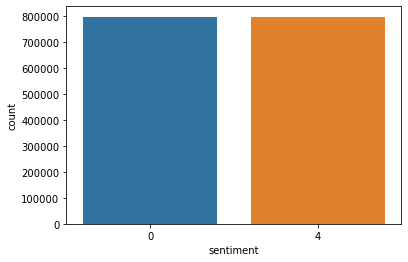
\includegraphics[scale=0.55]{images/train.png}
\end{center}
\caption{Distribución de las clases para datos de $training$}
\end{figure}

\vspace{2mm}
{\setlength{\parindent}{0cm}
En el \textbf{conjunto de Test} tenemos 498 tweets etiquetados como polaridad positiva (clase '4'), polaridad neutra (clase '2') y polaridad negativa (clase '0').}

\begin{figure}[htbp!]
\begin{center}
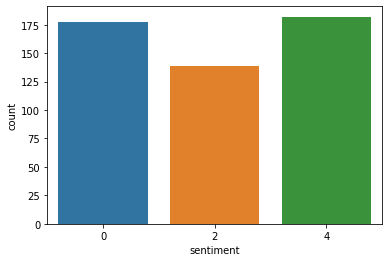
\includegraphics[scale=0.6]{images/test.png}
\end{center}
\caption{Distribución de las clases para datos de $test$}
\end{figure}

{\setlength{\parindent}{0cm}
Más adelante comentaremos que para el caso de evaluar los \textbf{modelos preentrenados}, que nos permiten clasificar documentos con estas 3 polaridades (positiva, neutra y negativa), \textbf{mantendremos todas las clases} de instancias del conjunto de datos de test para comprobar su funcionamiento en totalidad.}
\vspace{2mm}\\
Para el \textbf{resto de modelos} utilizados (en los que utilizaremos los datos de $training$ para el entrenamiento de éstos), \textbf{descartaremos} las instancias etiquetadas con polaridad \textbf{neutra} (clase '2') del conjunto de $test$, ya que en entrenamiento no tenemos de éstas.


\chapter{Descripción de los algoritmos}

\section{Métodos para la clasificación de documentos}

{\setlength{\parindent}{0cm}
La clasificación de un documento en función a la polaridad del sentimiento que expresa, puede llevarse a cabo de diversas formas. No hay un consenso (como en la mayoría de campos de la inteligencia artificial) sobre qué técnicas o algoritmos se deben usar para obtener mejores resultados en la clasificación de textos en unas situaciones u otras. }
\vspace{2mm}\\
Aun así, podemos diferenciar los dos grandes grupos en los se encuentran dichas técnicas:

\begin{enumerate}

\item \textbf{Métodos supervisados:} Se basa en el empleo de algoritmos de aprendizaje automático de tipo supervisado, ya que se parte de un conjunto de textos previamente etiquetados (se conoce su polaridad) con los que se entrena un modelo que será usado posteriormente para clasificar un nuevo conjunto de textos (que en este ámbito es conocida como colección documental o \textit{corpus}). 
\vspace{2mm}\\
Dichos algoritmos basan su funcionamiento en relaciones matemáticas creadas entre los elementos de entrenamiento. Éstos deben de ser representativos en cuanto a los elementos de test para el óptimo funcionamiento de éste (es el principal problema, no siempre se tiene un conjunto de entrenamiento lo suficientemente grande o bueno, a veces es difícil obtenerlo).


\item \textbf{Métodos no supervisados:} Resuelven el hecho de tener que contar con un conjunto de elementos preetiquetados (salva el problema de la dependencia del dominio). Estos métodos tratan de inferir la polaridad del sentimiento global de un documento a partir de la orientación semántica de las palabras o frases que lo conforman. Estos a su vez se dividen en: 

	\begin{enumerate}

	\item \textbf{Basados en diccionarios}: Hacen uso de un listado de palabras o frases junto a la polaridad que expresan, incluso con un grado de intensidad o fuerza de dicha polaridad. Tiene la desventaja de que a veces se pierde precisión ya que las palabras dependendiendo del contexto pueden tener una connotación más positiva o negativa, etc.
	\vspace{2mm}\\
	Ese problema se "resuelve" creando diccionarios concretos para un ámbito del lenguaje específico. Es decir el conjunto de palabras que lo forman se centra en un dominio concreto, por ejemplo: medicina. Pero aún dentro de un mismo ámbito podría seguir ocurriendo ésto y habría que hilar más fino en la construcción de los mismos.
	
	\item \textbf{Basados en relaciones lingüísticas}: Tratan de buscar ciertos patrones que expresen opiniones y sentimientos similares, con la mayor probabilidad posible, extrayendo las palabras que los formas para ser usadas posteriormente para clasificar textos mediante una función matematica que tenga en cuenta las palabras que lo contengan. 

	\end{enumerate}

\end{enumerate}

{\setlength{\parindent}{0cm}
El enfoque no supervisado es elegante pero necesita apoyarse de alguna forma en datos que aporten una cierta orientación y sirvan de base de conocimiento. Por ello nos \textbf{centraremos} en métodos de \textbf{aprendizaje supervisado}.}


\vspace{6mm}
\section{Random Forest}

{\setlength{\parindent}{0cm}
Random Forest es una combinación de árboles de decisión o predictores
tal que cada árbol depende de los valores de un vector aleatorio probado independientemente y con la misma
distribución para cada uno de éstos. Supone por tanto una mejora sobre los árboles de decisión clásicos y la técnica de \textit{bagging}.}

\begin{figure}[htbp!]
\centering
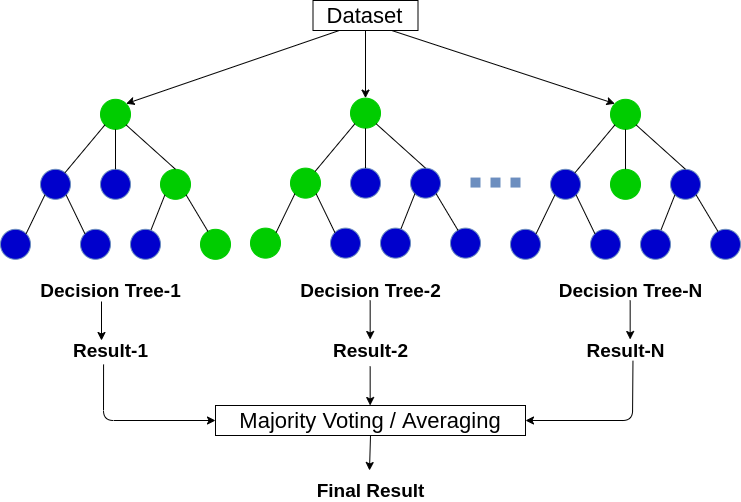
\includegraphics[scale=0.4]{images/rf.png}
\caption{Representación de Random Forest}
\end{figure}

{\setlength{\parindent}{0cm}
Este modelo permite tener múltiples árboles de decisión que son entrenados con una muestra de datos escogida con reemplazo a partir de la muestra original mediante \textit{bootstrap}. }
\vspace{2mm}
\\Además, cada árbol escoge un subconjunto de predictores que va a utilizar para intentar predecir, con el objetivo de evitar las correlaciones entre los distintos árboles, que era el principal problema de \textit{bagging} (si existe un una variable predictora fuerte, esta era utilizado casi siempre en la primera decisión del árbol, haciendo por tanto que la mayoría de árboles se parecieran).
\vspace{2mm}
\\Además, es un modelo que ofrece unos resultados muy buenos en general a la hora de clasificar, ya que obtiene un bajo sesgo y varianza al tener múltiples árboles y promediar entre ellos (que además sabemos que no están correlacionados).

\vspace{6mm}
\section{Máquinas de vectores de soporte}

{\setlength{\parindent}{0cm}
Las máquinas de vectores de soporte (del inglés, Support Vector Machine o SVM) son un grupo de algoritmos de aprendizaje supervisado en los que se trata de encontrar un hiperplano separador (denominado vector de soporte) que separe con la mayor distancia posible las distintas clases a las que pertenecen cada uno de los elementos.} 
\vspace{2mm}\\
De esta forma, el vector determina la frontera que sirve para clasificar un nuevo elemento. 
\vspace{2mm}\\
Cuenta con una serie de parámetros que permitirán optimizar los resultados durante el proceso de clasificación, uno de ellos es el \textit{kernel} y se utiliza cuando no es posible separar las muestras mediante una línea recta, plano o hiperplano de N dimensiones, permitiendo tal separación mediante otro tipo de funciones matemáticas como polinomios, funciones de base radial, etc. 
\vspace{2mm}\\
Otro parámetro conocido es  $regularization$ o $C$, que permite una fluctuación de manera que se consideren ciertos errores en la clasificación y se evite el sobreaprendizaje en la manera de lo posible.
\vspace{2mm}\\
Y otro de ellos es $gamma$ que determina la distancia máxima a partir de la cual una muestra pierde su influencia en la configuración del vector de soporte y $margin$ que es la separación entre el vector y las muestras de cada clase más cercanas al mismo. 

\vspace{6mm}
\begin{figure}[htbp!]
\centering
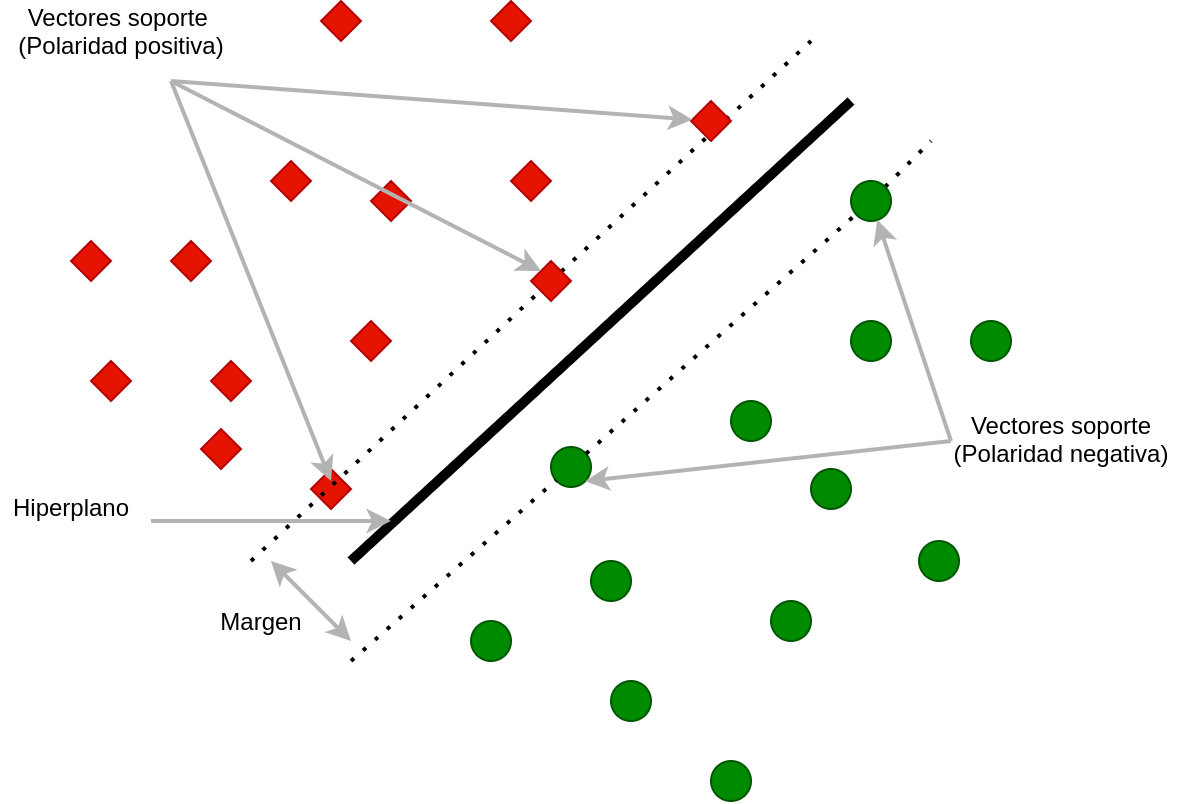
\includegraphics[scale=0.7]{images/SVM.png}
\caption{Representación de SVM para el problema}
\end{figure}



\section{Naive Bayes}

{\setlength{\parindent}{0cm}
La familia de algoritmos Naive Bayes se basan en el conocido \textit{Teorema de Bayes}:} \\

{\setlength{\parindent}{0cm}
\textit{Sea \{$A_1$, $A_2$, ... , $A_n$\} un conjunto de sucesos mútuamente excluyentes y exhaustivos, y tales que la probabilidad de cada uno de ellos es distinta de cero. Sea B un suceso cualquiera del que se conocen las probabilidades condicionales $P(B|A_i)$.}
\vspace{2mm}\\
Entonces la probabilidad de $P(A_i |B)$ viene dada por la expresión:}
\vspace{4mm}
\[ P(A_i | B) = \frac{P(B|A_i) * P(A_i)}{P(B)}  \]

\vspace{4mm}
{\setlength{\parindent}{0cm}
Para el caso de clasificación de textos, los sucesos son mútuamente excluyentes ya que no podemos considerar (en nuestro caso un tweet) que es de polaridad positiva y negativa al mismo tiempo y además son exhaustivos ya que esa calificación (positivo, negativo y neutro) son los únicos tipos que existen.}
\vspace{2mm}\\
Además consideraremos que las palabras de un mismo mensaje no tienen ningún tipo de relación entre sí y por lo tanto es indiferente la posición que tienen dentro del texto al que pertenecen. (Esta condición es conocida en este ámbito como la suposición de bolsa de palabras o \textit{bag of words}). 
\vspace{4mm}


\section{Métricas de evaluación}

{\setlength{\parindent}{0cm}
Para determinar el rendimiento de los resultados obtenidos por los distintos algoritmos, es necesario establecer unas métricas o medidas de evaluación que permitan evaluar de manera objetiva su eficacia a la hora de clasificar los ejemplos que se le proporiconen a éstos.}
\vspace{4mm}\\
Para ello, es importante tener en cuenta los cuatro posibles estados de un ejemplo clasificado, por ejemplo con respecto a una clase C:

\begin{enumerate}
\item \textbf{Verdaderos positivos} (True Positives o TP): son aquellos que han sido marcados de manera correcta como pertenecientes a la clase C.

\item \textbf{Falsos positivos} (False Positives o FP): son aquellos marcados como de clase C, pero que en realidad no pertenecen a dicha clase, es decir, han sido clasificados de forma incorrecta.

\item \textbf{Verdaderos negativos} (True Negatives o TN): son aquellos que no son de la clase C y han sido clasificados correctamente.

\item \textbf{Falsos negativos} (False Negatives o FN): son aquellos clasificados como no pertenecientes a la clase C, pero en realidad sí lo son y por tanto no se han clasificado correctamente.

\end{enumerate}

\vspace{6mm}
{\setlength{\parindent}{0cm}
Teniendo en cuenta los cuatro posibles estados anteriores, podemos definir las siguientes medidas que serán usadas para evaluar el rendimiento de nuestros modelos:}

\begin{enumerate}

\item \textbf{Exactitud o \textit{Accuracy}}: Es la medida de rendimiento más simple e intuitiva. Representa la relación entre las predicciones correctas sobre el total de las predicciones realizadas. 

\[  Accuracy = \frac{TP + TN}{TP + FP + TN + FN} \]

\vspace{4mm}
Podemos pensar que un modelo con mayor exactitud que otro es mejor. Eso sería así en el caso de que el número de elementos de cada clase es el mismo, es decir, el corpus está balanceado. En caso contrario, es necesario hacer uso de otro tipo de medidas como la precisión o la exhaustividad (valoran el rendimiento sobre clases individuales). 

\vspace{4mm}
\item \textbf{Precisión}: Es la razón entre el número de documentos clasificados correctamente como pertenecientes a la clase C y el número total de documentos que han sido clasificados por el modelo como de clase C. Mide la proporción de identificaciones positivas que son realmente correctas.

\[ Precision = \frac{TP}{TP + FP} \]

\vspace{4mm}
\item \textbf{Exhaustividad o \textit{Recall}}: Es la razón entre los documentos clasificados correctamente como pertenecientes a la clase C y la suma de todos los documentos de la clase C. Se puede entender como la capacidad que tiene el modelo de construir de manera correcta las clases.

\[ Recall = \frac{TP}{TP + FN} \]

\vspace{4mm}
\item \textbf{Media armónica ponderada o F-score}: Puede ser interpretado como un promedio ponderado de la \textit{precisión} y el \textit{recall} a través de un parámetro $\beta$ que permite otorgar una mayor importancia a una que otra, donde el rango de valores oscila entre 0 y 1. 

\[ F1 = (1 + \beta^{2})*  \frac{Precision * Recall}{(\beta^{2}*Precision) + Recall} \]

\vspace{4mm}
Se ayudará a penalizar los valores muy bajos en una u otra medida. Es frecuente que la precisión y el recall tengan el mismo peso en la fórmula, es decir, con un valor $\beta = 1$. A esta configuración se le conoce como \textbf{F1-score} y es el que \textbf{utilizaremos}.

\clearpage

Es de la forma:

\[ \frac{2*Precision*Recall}{Precision + Recall} \]
\vspace{4mm}
\end{enumerate}

{\setlength{\parindent}{0cm}
Para el caso en el que se cuenten con \textbf{más de 2 clases} (solo lo tendremos en cuenta al utilizar modelos preentrenados, ya que predeciremos tanto polaridad negativa, neutra y positiva. En nuestro conjunto de entrenamiento solo tenemos polaridad positiva y negativa), se debe \textbf{calcular} cada una de las \textbf{métricas anteriores} para \textbf{cada clase} y combinarlas  entre ellas para obtener una \textbf{medida global}. }
\vspace{2mm}\\
La función \texttt{classification\_report} de \textit{sklearn} nos proporciona: 

\begin{enumerate}

\item \textbf{Macro-averaging}: Se calculan las medias para cada una de las clases, tanto de precisión, recall y f1-score. Esta medida no tiene en cuenta el posible desbalanceo entre el número de ejemplos de cada clase. Por ejemplo para el caso de la precisión sería:

\[ Macro-precision = \frac{\sum_{i=1}^{n}Precision_i}{n} \]
\vspace{2mm}

\item \textbf{Weighted-averaging}: Resuelve el problema de tener un $corpus$ desbalanceado y con más de dos clases. Se pondera cada componente de la fórmula en base al peso que cada clase tiene dentro del sistema. De nuevo, para el caso de la precisión sería: 

 \[ Weighted-precision = \frac{\sum_{i=1}^{n}Precision_i * P_i}{n} \]

\end{enumerate}


\vspace{4mm}
{\setlength{\parindent}{0cm}
Comentar que los algoritmos anteriormente nombrados serán entrenados mediante \textbf{validación cruzada} o \textit{cross-validation}, de forma que se reducirá la dependencia entre la partición de los datos usada para la fase de entrenamiento y test. }
\vspace{2mm}\\
Se dividirá el conjunto de documentos o \textit{corpus} en 5 particiones de iugal tamaño, de forma que que 4 serán para entrenar el modelo y el sobrante para la evaluación. Esto se repetirá 5 veces de forma que al final se promediará el valor de las métricas para tener una medida más robusta. 



\chapter{Estudio experimental}

Para abordar el problema, se nos han propuesto una serie de aproximaciones en orden creciente de complejidad:

\begin{itemize}

\item Comenzaremos utilizando modelos de análisis de sentimientos ya preentrenados.
\item A continuación construiremos nuestro propio método de análisis de sentimientos (crearemos un clasificador haciendo uso de los algoritmos explicados anteriormente y aplicando un preprocesado a los datos para mejorar los resultados).
\item Y por último (como ampliación de la práctica) utilizaremos modelos mucho más avanzados.
\end{itemize}


\section{Empleo de métodos de análisis de sentimientos preentrenados (SAMs)}

{\setlength{\parindent}{0cm}
Estos métodos ya han sido preentrenados con un conjunto de textos que representan de forma general el tipo de polaridad (positiva, negativa, neutra) que puede expresar una oración o documento. }
\vspace{2mm}\\
No será necesario entrenar con nuestros datos, sólamente tendremos que utilizar los datos de test para predecir directamente la polaridad que expresan nuestros tweets.

\subsection{VaderSentiment}

{\setlength{\parindent}{0cm}
VADER \textit{(Valence Aware Dictionary and sEntiment Reasoner)} es una herramiento de análisis de sentimientos basada en reglas y léxico que está específicamente en sintonía con los sentimientos expresados en las redes sociales. Es completamente de código abierto y se instala como una librería más para python a través de $pip$.}
\vspace{2mm}\\
La puntuación $compound$ se calcula sumando las puntuaciones de valencia de cada palabra en el léxico, se ajusta de acuerdo con las reglas y luego se normaliza para estar entre -1 (extremo más negativo) y +1 (extremo más positivo).
\vspace{2mm}\\
Esta es la métrica más útil si desea una única medida unidimensional de sentimiento para una oración determinada.
\clearpage
El \textbf{significado} de dicha \textbf{puntuación} es el siguiente:

\begin{itemize}
\item sentimiento positivo : $compound >= 0,05 $
\item sentimiento neutral : $compound > -0,05$ y $compound < 0,05$
\item sentimiento negativo : $compound <= -0,05$  
\end{itemize}

{\setlength{\parindent}{0cm}
Los \textbf{resultados obtenidos} para el conjunto de $test$ han sido los siguientes: }

\begin{table}[htbp!]
\centering
\scalebox{1.0}{\begin{tabular}{|c|c|c|c|}
\hline
\rowcolor{lightgray}
Polaridad & Precision & Recall & F1-score \\ \hline \hline 

Negativo &  0.84  &   0.64  &   0.73 \\\hline
Neutro   &  0.67  &   0.70  &   0.68 \\\hline
Positivo &  0.68  &   0.81  &   0.74 \\\hline \hline

\rowcolor{lightgray}
Macro avg     & 0.73   &  0.72  &  0.72  \\\hline
\rowcolor{lightgray}
Weighted avg  & 0.73   &  0.72  &  0.72  \\\hline \hline

\rowcolor{lightgray}
Accuracy & \multicolumn{3}{|r|}{0.72}  \\\hline

\end{tabular}}
\caption{Resultados para VaderSentiment}
\end{table}


\subsection{TextBlob}

{\setlength{\parindent}{0cm}
TextBlob es una biblioteca de Python (2 y 3) para procesar datos textuales. Proporciona una API simple para sumergirse en tareas comunes de procesamiento del lenguaje natural (NLP), como etiquetado de parte del discurso, extracción de frases nominales, análisis de sentimientos, clasificación, traducción y más.}
\vspace{2mm}\\
{\setlength{\parindent}{0cm}
Los \textbf{resultados obtenidos} para el conjunto de $test$ han sido los siguientes: }

\vspace{2mm}
\begin{table}[htbp!]
\centering
\scalebox{1.0}{\begin{tabular}{|c|c|c|c|}
\hline
\rowcolor{lightgray}
Polaridad & Precision & Recall & F1-score \\ \hline \hline 

Negativo &  0.81  &   0.48  &   0.60 \\\hline
Neutro   &  0.59  &   0.70  &   0.64 \\\hline
Positivo &  0.63  &   0.79  &   0.70 \\\hline \hline 

\rowcolor{lightgray}
Macro avg     & 0.68   &  0.66  &  0.65  \\\hline
\rowcolor{lightgray}
Weighted avg  & 0.68   &  0.65  &  0.65  \\\hline \hline

\rowcolor{lightgray}
Accuracy & \multicolumn{3}{|r|}{0.65}  \\\hline

\end{tabular}}
\caption{Resultados para TextBlob}
\end{table}

A la vista de los resultados, pese a no haber visto una sola muestra de entrenamiento, los resultados son aceptables, sobretodo en el caso de VaderSentiment (la cual está entrenada con textos de redes sociales) y es más afín a nuestro problema.
\vspace{2mm}\\
Comentar que TextBlob también nos permitía a través de su API entrenar un modelo de Naive Bayes (ahora sí utilizando nuestros datos de entrenamiento) con el que hemos obtenido un precisión del 72\% aprox. Los resultados serán comentados más en profundidad en el análisis que haremos más adelante. 

\clearpage

\section{Creación de un propio método de análisis de sentimientos}

{\setlength{\parindent}{0cm}
La construcción de un clasificador de documentos de texto basado en un sistema de aprendizaje automático consta de varias etapas. En primer lugar es necesario preparar los datos del \textit{corpus} antes de pasárselos a los algoritmos. Se deben limpiar y normalizar de forma que se reduzca o eliminen datos innecesarios para el aprendizaje o que puedan influir de manera negativa en éste.}
\vspace{2mm}\\
A continuación cada uno de los tweets se someterá a un proceso de \textbf{tokenización}, el cual dividiremos el texto en unidades de significado conocidas como \textit{tokens} (suelen ser palabras).\vspace{2mm}\\
A partir de ellos se extraerán las características que representen a los mensajes y se aplicarán métodos para reducir su número, como podría ser la aunación de términos morfológicamente similares para reducir su número. Finalmente se ponderarán las características en función de la importancia que se les quiera dar y con ellas se entrenarán los clasificadores. 

\vspace{4mm}
\begin{figure}[htbp!]
\centering
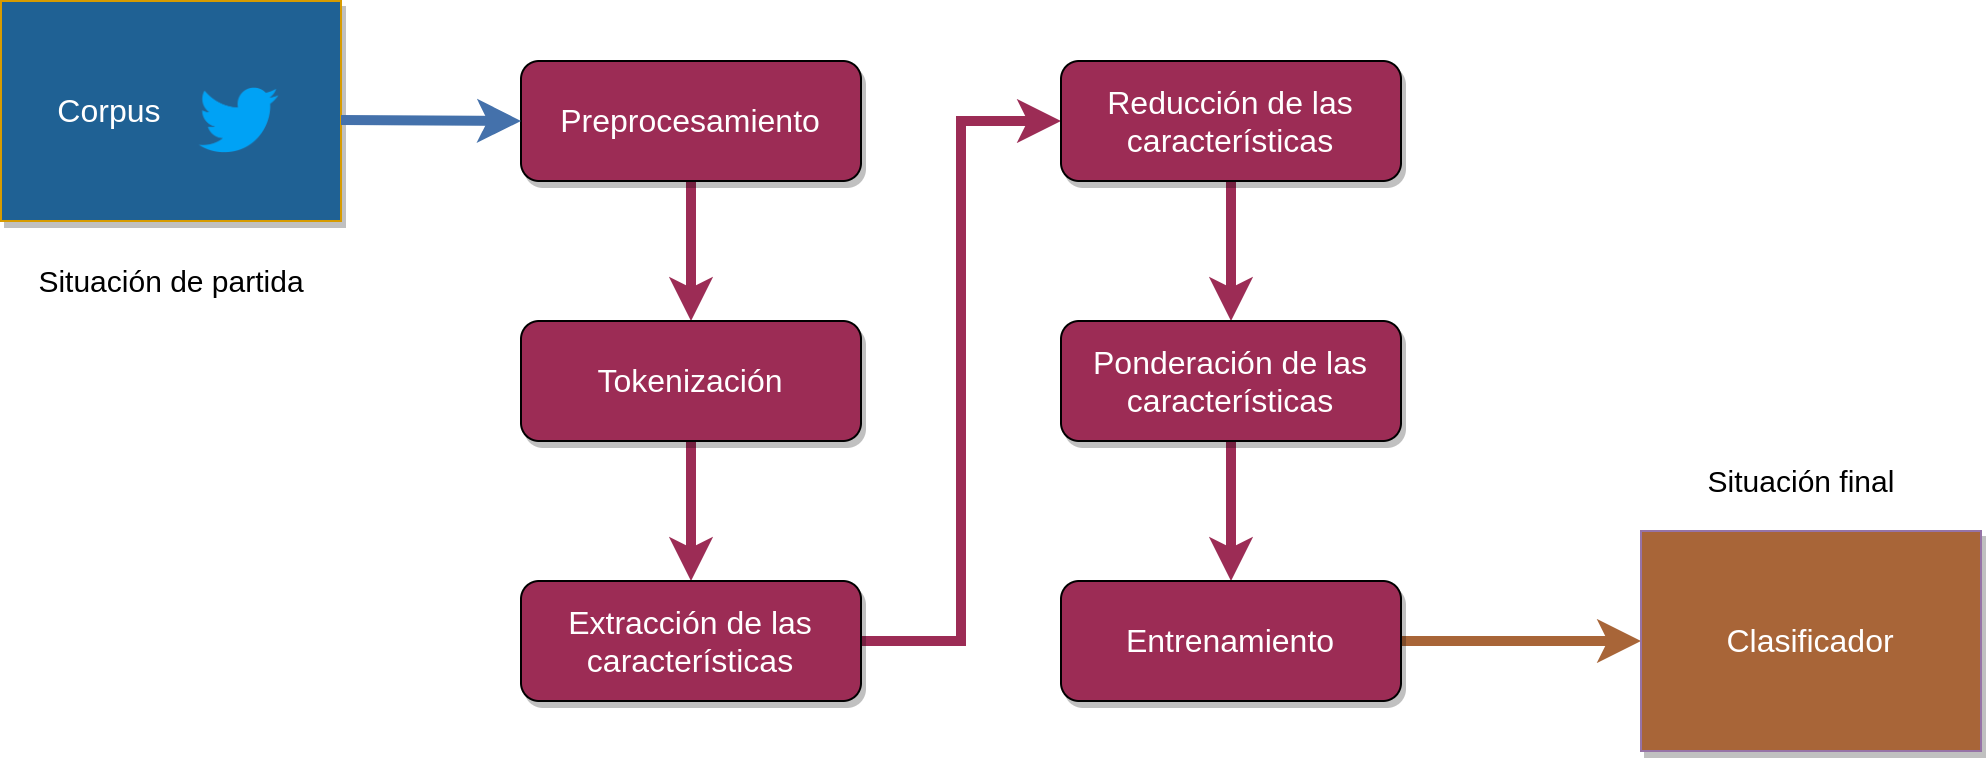
\includegraphics[scale=0.65]{images/Fases_SA.png}
\caption{Fases para la creación del clasificador}
\end{figure}
\vspace{2mm}


\subsection{Preprocesamiento}

{\setlength{\parindent}{0cm}
Partimos de una colección de tweets en los que tenemos todo tipo de información: urls, menciones, hashtags, repeticiones de caracteres, mezcla de letras mayúsculas y minúsculas etc. El objetivo de esta fase es tratar de limpiar y normalizar los datos que puedan influir de manera negativa a la hora de clasificar. \cite{Jain} }
\vspace{2mm}\\
A continuación comentamos una serie de tratamientos que hemos aplicado a cada uno de los tweets de forma que se limpien esos datos pero sin provocar una pérdida excesiva de la polaridad de los mismos:

\begin{enumerate}

\item \textbf{Decodificando HTML}: Parece que la codificación HTML no se ha convertido a texto y en algunos casos se encuentran terminaciones como '\&amp' y '\&quot'. Por lo que haremos uso de la librería \textbf{BeautifulSoup} para extraer preprocesar esos tweets que contengan información de este tipo.

\item \textbf{Eliminando @mention}: La segunda parte del preprocesamiento será eliminar las menciones que unos usuarios hacen a otros. Esta información no aportará nada de valor a la hora de construir un modelo de análisis de sentimiento. Utilizaremos una expresión regular. 

\item \textbf{Eliminando URL links}: Sucede de forma similar que con las menciones, es información relevante en el tweet pero para fines de análisis de sentimientos, podemos ignorarlos. Utilizaremos una expresión regular.

\item \textbf{Hashtags y números}: A veces, el texto utilizado con un hashtag puede proporcionar información útil sobre el tweet. Puede ser un poco arriesgado deshacerse de todo el texto junto con el hashtag. Simplemente eliminaremos el '\#'. Haré esto en el proceso de limpieza de todos los caracteres que no son letras, incluidos los números. 

\item \textbf{Normalización a minúsculas}: Una misma palabra escrita de forma completa en mayúsculas y en minúsculas es tratada de forma distinta por un algoritmo de aprendizaje automático. Para evitar que esto suceda, convertiremos todos los mensajes a su equivalente en letras minúsculas, de la misma forma que haría un \textit{LowerCaseFilter}.

\end{enumerate}

De forma que la función para la limpieza del tweet nos queda de la forma: 

\vspace{2mm}
\begin{lstlisting}[language=Python]
from bs4 import BeautifulSoup
import re

pat1 = r'@[A-Za-z0-9]+'
pat2 = r'https?://[A-Za-z0-9./]+'
combined_pat = r'|'.join((pat1, pat2))

def tweet_cleaner(text):
    
    # HTML Decoding
    soup = BeautifulSoup(text, 'lxml')
    
    # @Menciones, URL links
    souped = soup.get_text()
    stripped = re.sub(combined_pat, '', souped)
    try:
        clean = stripped.decode("utf-8-sig").replace(u"\ufffd", "?")
    except:
        clean = stripped
    
    # Hashtag, numeros
    letters_only = re.sub("[^a-zA-Z]", " ", clean)
    
    # LoweCaseFilter
    lower_case = letters_only.lower()
    
    words = tok.tokenize(lower_case)
    
    return (" ".join(words)).strip()

\end{lstlisting}


\subsection{Tokenización}

{\setlength{\parindent}{0cm}
Una vez completado el proceso de normalización de los mensajes, la siguiente etapa es la de tokenización. Consiste en dividir el texto en unidades más pequeñas llamadas tokens las cuales tienen un significado propio y que normalmente suelen ser cada una de las palabras del mensaje. Por lo tanto \textbf{separaremos } los \textbf{términos} del tweet por \textbf{espacios en blanco}. }

\vspace{4mm}
\subsection{Extracción de las características}

{\setlength{\parindent}{0cm}
A partir de los tokens obtenidos en el paso anterior, se define una manera de representar los mensajes, creando así las características de cada tweet. Lo habitual en clasificación de documentos es hacer uso del modelo de bolsa de palabras ya mencionario anteriormente (también conocido como del inglés como \textit{bag of words}) donde cada mensaje se representa mediante sus tokens \textbf{sin tener en cuenta} el \textbf{orden} en los que éstos aparecen. En nuestro caso \textbf{cada característica} será un \textit{unigrama} o token individual. }

\vspace{4mm}
\subsection{Reducción de las características}

{\setlength{\parindent}{0cm}
Esta fase suele ser opcional y el objetivo es reducir la dimensionalidad o el número de características del $corpus$ mediante la la \textbf{eliminación} de algunos de ellos, \textbf{aunación} de tokens morfológicamente similares, la \textbf{conversión} de tokens parecidos a otro token más general.}
\vspace{2mm}\\
Existen técnicas para llevar a cabo cada una de esas tareas comentadas:

\begin{enumerate}

\item \textbf{Eliminación de palabras vacías}: En todos los idiomas hay un conjunto de palabras pequeño que suele tener una frecuencia muy alta y que por norma general sirven para construir las oraciones pero que carecen de información. Estas palabras son las preposiciones, conjunciones, artículos, etc. 
\vspace{2mm}\\
Se define una lista con dichas palabras, conocidas como \textit{stopwords} y serán eliminadas de cada uno de los tweets, de forma que se reducirá el número de características del mismo. 

\item \textbf{Stemming}: Es un método de normalización lingüística que transforma cada palabra a su raíz por medio de la supresión de prefijos, sufijos e infijos. Por ejemplo las palabras: perro, perrito, perritas se reduciría a una misma raiz perr.


\item \textbf{Lematización}: Es otro método de normalización lingüística en el que cada palabra se transforma en su lema mediante el uso de un diccionario y un proceso de análisis morfológico. 
\vspace{2mm}\\
Por ejemplo podría considerarse el cambio de género o número a una misma forma. Se trata de reducir la variabilidad de una palabra. Es más costoso que el stemming, pero como resultado tenemos un reducción más fina de los términos. 

\end{enumerate}

De forma que la función para la reducción del tweet nos queda de la forma: 

\vspace{2mm}
\begin{lstlisting}[language=Python]
# English Stopwords
import nltk
nltk.download('stopwords')
stop_words = set(stopwords.words('english'))

def preprocesar_texto_tweet(tweet):
    
    # Ya los teniamos convertidos a minuscula
    
    # Eliminamos las palabras vacias (Filtramos aquellas que no lo son) 
    tweet_tokens = word_tokenize(tweet)
    filtered_words = [word for word in tweet_tokens if word not in stop_words]
    
    # Stemming
    ps = PorterStemmer()
    stemmed_words = [ps.stem(w) for w in filtered_words]
    
    # Lematizacion
    lemmatizer = WordNetLemmatizer()
    lemma_words = [lemmatizer.lemmatize(w, pos='a') for w in stemmed_words]
    
    return " ".join(lemma_words)
\end{lstlisting}
\vspace{2mm}
A continuación mostramos el top de los 50 términos más frecuentes utilizados en tweets con polaridad negativa sin considerar la reducción de características y tras considerarla:


\begin{figure}[htbp!]
\begin{center}
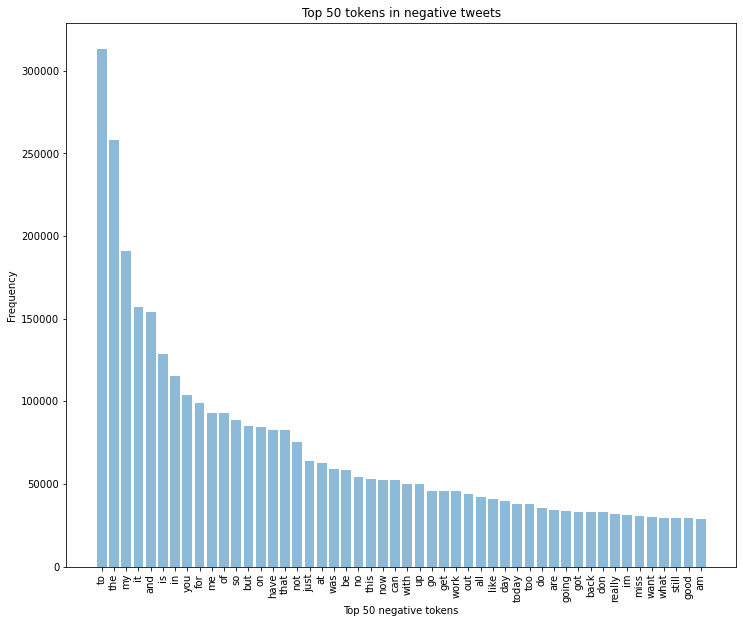
\includegraphics[scale=0.3]{images/neg.png}
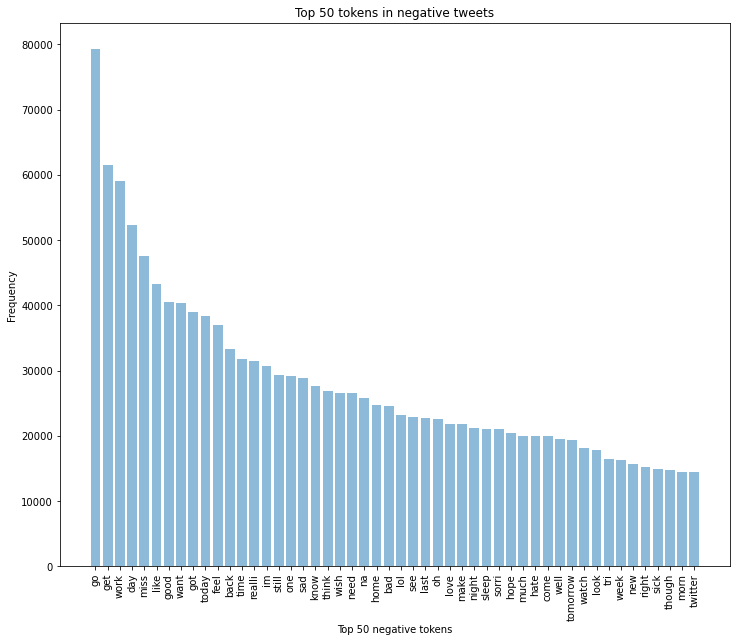
\includegraphics[scale=0.3]{images/neg_clean.png}
\end{center}
\caption{Top 50 términos negativos antes y después de preprocesar}
\end{figure}

{\setlength{\parindent}{0cm}
Podemos observar que antes aparecían palabras como: \textit{to, the, my, it, and} que son \textbf{palabras } carentes de significado o \textbf{vacías} (stopwords) y no reflejan el sentimiento negativo. }
\vspace{2mm}\\
\textbf{Tras preprocesar} podemos ver como entre las palabras más frecuentes aparecen: \textit{get, work, miss, feel, sad, wish, bad} las cuales son mucho más \textbf{representativas} para expresar la \textbf{polaridad negativa}.

\clearpage

{\setlength{\parindent}{0cm}
De la misma forma ocurre con los 50 términos más frecuentes utilizados en tweets que con polaridad positiva. De la misma forma que antes, las gráficas resultantes son:}

\begin{figure}[htbp!]
\begin{center}
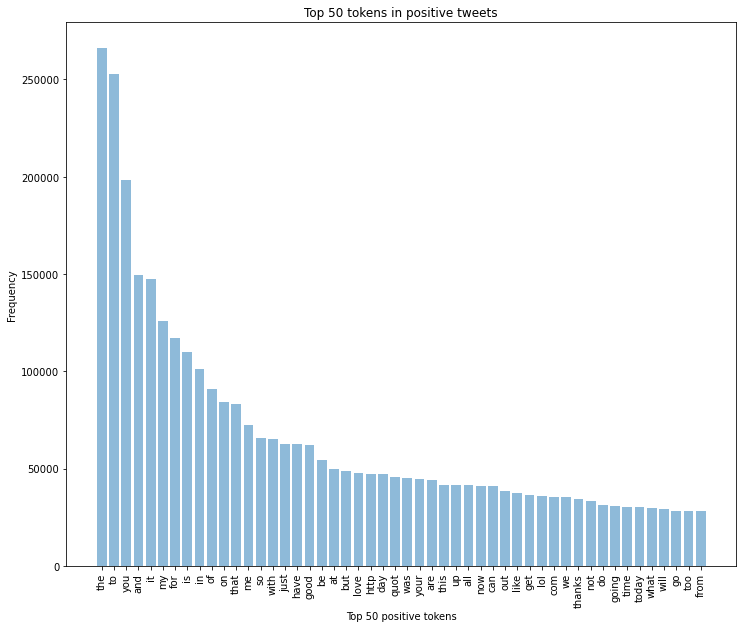
\includegraphics[scale=0.3]{images/pos.png}
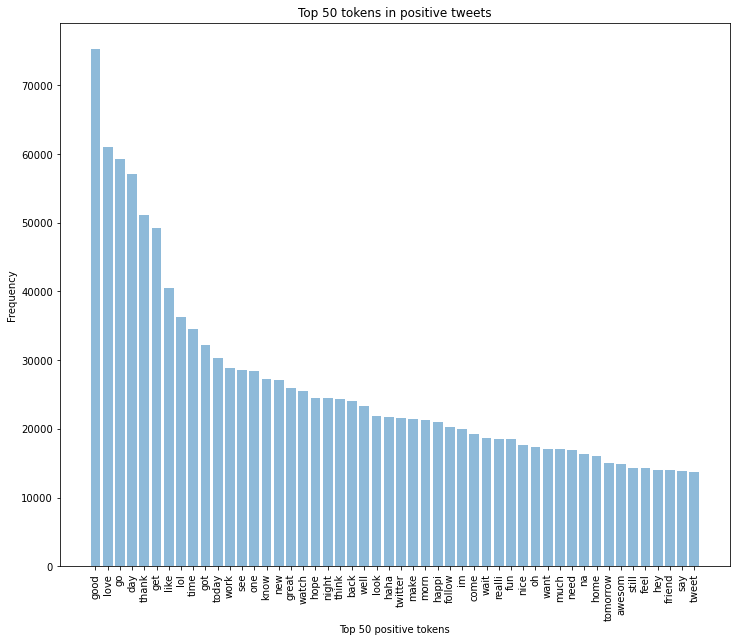
\includegraphics[scale=0.3]{images/pos_clean.png}
\end{center}
\caption{Top 50 términos positivos antes y después de preprocesar}
\end{figure}

{\setlength{\parindent}{0cm}
Podemos observar que vuelven a aparecer de hecho las mismas palabras como: \textit{the, to, you, it, and} que son \textbf{palabras} \textbf{vacías} y además de no reflejar el sentimiento positivo, coinciden con las negativas y por lo tanto pueden causar confusión para el clasificador. }
\vspace{2mm}\\
Tras preprocesar podemos ver como entre las palabras más frecuentes aparecen: \textit{good, love, thank, like, lol, great} las cuales son mucho más \textbf{representativas} para expresar la \textbf{polaridad positiva}.
\vspace{4mm}\\
La \textbf{reducción de la dimensionalidad} es bastante notable. Como ya comentaremos más adelante, utilizaremos un total de 6000 instancias para el entrenar los clasificadores. \\
Tras obtener el esquema tf-idf para cada uno de los documentos, obtenemos una matriz de:  6000 rows × 12554 columns.
\vspace{2mm}\\
Una vez preprocesado todos los datos, obtenemos una matriz de: 6000 rows × 7649 columns, 
lo que supone una reducción de dimensionalidad de un \textbf{39\%} y por lo tanto los \textbf{tiempos de ejecución} y los \textbf{resultados} como veremos más adelante, \textbf{mejorarán} significativamente. 
\vspace{4mm}

\subsection{Ponderación de las características}

{\setlength{\parindent}{0cm}
Las características extraídas pueden ser consideradas con la misma importancia o podemos asignarle distintos pesos en función de algún tipo de criterio, como por ejemplo la frecuencia de aparición de éstas en el propio tweet o en relación con la totalidad e los tweets.\vspace{2mm}\\
Existen distintos métodos de ponderación, los cuales se han visto con más profundidad en la asignatura de Recuperación de Información, pero aquí voy a mostrar directamente el más famoso y utilizado en el ámbito de \textit{Text mining} e \textit{Information retrieval}, que es el esquema de \textbf{ponderación TF-IDF}. 
\vspace{2mm}\\
Definimos a continuación los dos conceptos que componen a dicho esquema de ponderación: }
\vspace{2mm}

\begin{itemize}

\item \textbf{Term Frequency} o TF:

\[ tf_{ij} = \frac{n_{ij}}{\sum_{k} n_{kj}}  \]

{\setlength{\parindent}{0cm}
La frecuencia del término $i$ en el documento $j$ se define como el número de veces que aparece una palabra en un documento dividido por el número total de palabras del documento. }


\item \textbf{Inverse Document Frequency} o IDF:

\[ idf_i = log \left( \frac{N}{df_t} \right) \]

{\setlength{\parindent}{0cm}
La frecuencia documental inversa de un término $i$ se define como el logaritmo del número de documentos del $corpus$ dividido entre el número de documentos en los que aparece el término $i$.} \vspace{2mm}\\
Favorece por tanto a las palabras que aparecen en pocos documentos y penaliza a aquellas que suelen aparecer en la mayoría (son las que no nos ayudan a discriminar los documentos). 

\end{itemize}
\vspace{2mm}

{\setlength{\parindent}{0cm}
Finalmente, el \textbf{esquema TF-IDF}, que será la ponderación de un término $i$ en un documento $j$, se define como el producto de ambos conceptos:}

\[ w_{ij} = tf_{ij} \times log \left( \frac{N}{df_t} \right) \] 

\vspace{2mm}
{\setlength{\parindent}{0cm}
No será necesario calcular éstos datos de forma manual, podemos hacer uso de la clase
\texttt{TfidfVectorizer} proporcionada por $sklearn$. }
\vspace{4mm}

\section{Comparación y análisis de los modelos empleados}

{\setlength{\parindent}{0cm}
Al haber 1.6 millones de tweets, los tiempos de ejecución pueden dispararse, por lo
que emplearemos, como se nos ha recomendado, un subconjunto representativo y
balanceado del conjunto de Train.}
\vspace{2mm}\\
En concreto, vamos a utilizar una pequeña submuestra de 6000 instancias (3000 para cada una de las polaridades, positiva y negativa). He intendado hacerlo con 4000 para cada una de ellas, pero la memoria RAM se llena muy rápido y el ordenador se quedaba colgado hasta tener que apagarlo forzósamente. 
\vspace{2mm}\\
A continuación, mostramos las tablas con los resultados de las métricas de evaluación obtenidas para cada uno de los modelos considerados (utilizando y sin utilizar el preprocesamiento anteriormente comentado).
\clearpage

\subsection{Tablas con los resultados}

\vspace{12mm}

\begin{table}[htbp!]
\centering
\scalebox{1.0}{\begin{tabular}{|c|c|c|c|c|c|c|}
\hline
\rowcolor{lightgray}
& \multicolumn{3}{|c|}{Sin preprocesamiento} & \multicolumn{3}{|c|}{Con preprocesamiento} \\\hline

\rowcolor{lightgray}
Polaridad & Precision & Recall & F1-score & Precision & Recall & F1-score \\ \hline \hline 

Negativo &  0.68  &   0.67  &   0.67 &  0.79 & 0.68 & 0.70 \\\hline
Positivo &  0.68  &   0.70  &   0.69 &  0.69 & 0.80 & 0.77 \\\hline \hline

\rowcolor{lightgray}
Macro avg     & 0.68   &  0.68  &  0.68  & 0.74   &  0.74  &  0.73 \\\hline
\rowcolor{lightgray}
Weighted avg  & 0.68   &  0.68  &  0.68  & 0.74   &  0.74  &  0.73 \\\hline \hline
\rowcolor{lightgray}
Accuracy & \multicolumn{3}{|r|}{0.68}  & \multicolumn{3}{|r|}{0.74} \\\hline

\end{tabular}}
\caption{Resultados para Random Forest}
\end{table}


\vspace{10mm}


\begin{table}[htbp!]
\centering
\scalebox{1.0}{\begin{tabular}{|c|c|c|c|c|c|c|}
\hline
\rowcolor{lightgray}
& \multicolumn{3}{|c|}{Sin preprocesamiento} & \multicolumn{3}{|c|}{Con preprocesamiento} \\\hline

\rowcolor{lightgray}
Polaridad & Precision & Recall & F1-score & Precision & Recall & F1-score \\ \hline \hline 

Negativo &  0.73  &   0.68  &   0.70 &  0.80 & 0.63 & 0.70 \\\hline
Positivo &  0.71  &   0.75  &   0.73 &  0.70 & 0.85 & 0.77 \\\hline \hline

\rowcolor{lightgray}
Macro avg     & 0.72   &  0.72  &  0.72  & 0.75   &  0.75  &  0.75 \\\hline
\rowcolor{lightgray}
Weighted avg  & 0.72   &  0.72  &  0.72  & 0.75   &  0.75  &  0.75 \\\hline \hline
\rowcolor{lightgray}
Accuracy & \multicolumn{3}{|r|}{0.72}  & \multicolumn{3}{|r|}{0.75} \\\hline

\end{tabular}}
\caption{Resultados para SVM}
\end{table}

\vspace{10mm}


\begin{table}[htbp!]
\begin{center}
\scalebox{1.0}{\begin{tabular}{|c|c|c|c|c|c|c|}
\hline
\rowcolor{lightgray}
& \multicolumn{3}{|c|}{Sin preprocesamiento} & \multicolumn{3}{|c|}{Con preprocesamiento} \\\hline

\rowcolor{lightgray}
Polaridad & Precision & Recall & F1-score & Precision & Recall & F1-score \\ \hline \hline 

Negativo &  0.73  &   0.74  &   0.73 &  0.77 & 0.70 & 0.73 \\\hline
Positivo &  0.74  &   0.73  &   0.74 &  0.73 & 0.80 & 0.76 \\\hline \hline

\rowcolor{lightgray}
Macro avg     & 0.74   &  0.74  &  0.74  & 0.74   &  0.75  &  0.74 \\\hline
\rowcolor{lightgray}
Weighted avg  & 0.74   &  0.74  &  0.74  & 0.74   &  0.75  &  0.74 \\\hline \hline
\rowcolor{lightgray}
Accuracy & \multicolumn{3}{|r|}{0.74}  & \multicolumn{3}{|r|}{0.74} \\\hline

\end{tabular}}
\caption{Resultados para Naive Bayes}
\end{center}
\end{table}

\clearpage

A la vista de los resultados obtenidos, lo primero que nos llama la atención es que en \textbf{todos} los \textbf{algoritmos}, en la mayoría de métricas, los \textbf{resultados mejoran} cuando aplicamos el \textbf{preprocesamiento} a los documentos de partida. Las diferencias más grandes en cuanto a \textit{accuracy} nos referimos, se pueden observar sobretodo en Random Forest y también en SVM. 
\vspace{2mm}\\
Naive Bayes parece ser igual de robusto indiferentemente si aplicamos o no el preprocesados a los datos. Sin embargo, si nos fijamos el preprocesamiento ayuda sobretodo a \textbf{mejorar la clasificación} de los casos \textbf{positivos}. 
\vspace{2mm}\\
Esto ocurre en todos los casos, se obtiene un \textit{recall} a la hora de clasificar los tweets con \textbf{polaridad positiva} un 15\% superior tras preprocesar en Random Forest, un 10\% superior en SVM y un 7\% superior en Naive Bayes.
\vspace{2mm}\\
A diferencia del \textit{recall} para los tweets con \textbf{polaridad negativa} que baja un 5\% en todos los algoritmos aproximadamente. Esto puede ocurrir bien porque el subconjunto de entrenamiento de nuestro dataset es bastante pequeño y no es demasiado representativos para los casos negativos de aquellos términos que expresan la polaridad negativa.
\vspace{4mm}\\
Si comparamos los resultados de \textit{accuracy} obtenidos en nuestros clasificadores propios contra los modelos preentrenados (VaderSentiment y TextBlob) que comentamos anteriormente, podemos observar que \textbf{nuestros modelos} ofrecen \textbf{mejor comportamiento} obtniendo unos resultados de media un 10\% superiores respecto a TextBlob y un 3\% superiores a VaderSentiment.
\vspace{2mm}\\
A continuación mostramos en una tabla todos los clasificadores/modelos empleados junto a su accuracy

\begin{table}[htbp!]
\begin{center}
\scalebox{1.0}{\begin{tabular}{|c|c|}
\hline
\rowcolor{lightgray}
Clasificador & \textit{Accuracy} \\\hline
VaderSentiment & 0.72 \\\hline
TextBlob & 0.65 \\\hline
Random Forest & 0.74 \\\hline
\rowcolor{lightgray}
Support Vector Machine & 0.75 \\\hline
Naive Bayes & 0.74 \\\hline
\end{tabular}}
\end{center}
\end{table}

Comentar que VaderSentiment, pese a no haber sido entrenado con nuestros datos de tweets, obtiene buenos resultados ya que este clasificador está en sintonía con los sentimientos expresados en las redes sociales, por lo tanto la forma de expresión de los usuarios de Tweeter le es familiar.
\vspace{2mm}\\
En cuanto a propios clasificadores, los mejores resultados los hemos obtenido con SVM (en concreto con el \textit{kernel} de base radial o \textit{rbf}) y tras hacer una \textbf{búsqueda} de los \textbf{mejores parámetros} con \texttt{GridSearchCV}. Obtenemos aprox. un 76\% considerando el modelo SVC(C=200, class\_weight='balanced', gamma=0.001).
\vspace{2mm}\\
Una buena ídea es combinar un conjunto de clasificadores (\textit{ensemble}) con el fin de mejorar la precisión de las estimaciones que se pueden lograr utilizando un solo clasificador \cite{Rokach}. \\También mejorar el rendimiento del clasificador SVM mediante el desarrollo de métodos de conjunto con un sistema de clasificación de polaridad basado en léxico o diccionarios \cite{Kennedy}. 


\clearpage

\begin{comment}
Este es el único caso en el que apenas se notan los cambios al preprocesar, pero sí podemos ver
que tenemos una mejor tasa de acierto a la hora de predecir los casos positivos tras el preprocesado ya que el \textit{recall} es superior, aunque de media tenemos el mismo valor 0.74
\end{comment}


\section{Modelos más avanzados}

A continuación, como ampliación de la práctica, \textbf{comentaremos} a grandes rasgos la \textbf{teoría} subyacente por debajo de estos modelos y formas de representación del texto que son más complejas pero con mejor comportamiento en general. Además \textbf{incluyo en la entrega el código} en \textit{jupyter-notebook} de los experimentos realizados que comentaré más adelante.


\subsection{Word2vec}

Es una herramienta que proporciona una implementación eficiente de las arquitecturas continuas de bolsa de palabras o \textit{bag of words} y omisión de la gramática para computar \textbf{representaciones vectoriales} de palabras que logran capturar el \textbf{significado semántico} de las mismas (a diferencia del esquema de representación tf-idf que consideran las palabras por separado como características).
\vspace{2mm}\\
Word2vec toma un $corpus$ de texto como entrada y produce los vectores de palabra como salida. 
Primero se \textbf{construye un vocabulario} a partir de los datos del texto de entrenamiento y luego se \textbf{aprende la representación vectorial}. de las palabras. Las palabras resultantes pueden utilizarse como características para entrenar nuestros modelos de aprendizaje automático. 
\vspace{2mm}\\
Para entender cómo funciona la representación vectorial de una palabra, y poder encontrar palabras cercanas o similares a otras, se utiliza como concepto de \textbf{distancia} la \textbf{similitud coseno}. Por ejemplo si se ingresa la palabra 'España', las palabras similares a ésta estarán cerca de ella, como podrían ser 'Francia', 'Alemania' etc.
\vspace{2mm}\\
De la misma forma ocurriría con adjetivos. En la siguiente imagen se muestra como \textbf{aquellos} que \textbf{son positivos} están \textbf{más cerca entre sí}, de igual forma ocurre con los negativos. 


\vspace{4mm}
\begin{figure}[htbp!]
\centering
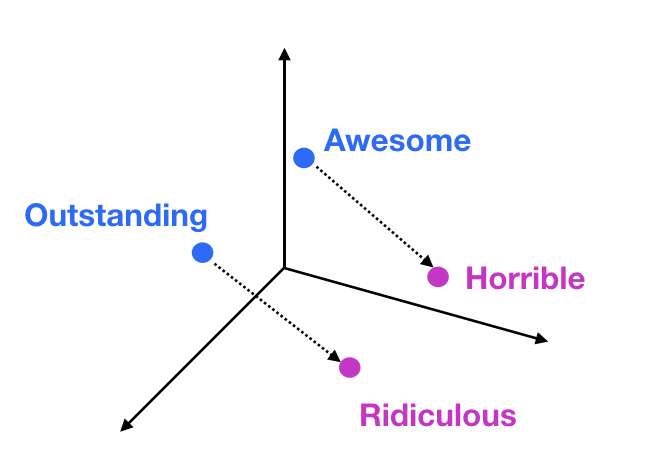
\includegraphics[scale=0.4]{images/w.png}
\caption{Representación word2vec}
\end{figure}
\vspace{2mm}


Para entrenar este modelo, se toman en consideración las palabras que rodean esa palabra de tamaño de ventana particular. Hay diferentes formas de derivar los vectores de incrustación de palabras. Word2vec es uno de esos métodos donde se utiliza el modelo de incrustaciones neuronales para aprender eso. Utiliza las siguientes \textbf{dos arquitecturas} para lograr esto.

\begin{itemize}

\item \textbf{Bolsa Contínua de Palabras o CBOW}: del inglés Continuous Bag of Words, se trata de un modelo que predice la palabra en consideración con las palabras dadas como contexto dentro de una ventana específica. La capa oculta tiene un número de dimensiones igual a las necesarias para representar la palabra actual en la capa de salida. 
\vspace{2mm}\\
En el siguiente ejemplo se muestra una ventana de tamaño 2 para predecir el vector de la palabra 'awesome' dada la oración: 'Restaurant was awesome this time’


\vspace{4mm}
\begin{figure}[htbp!]
\centering
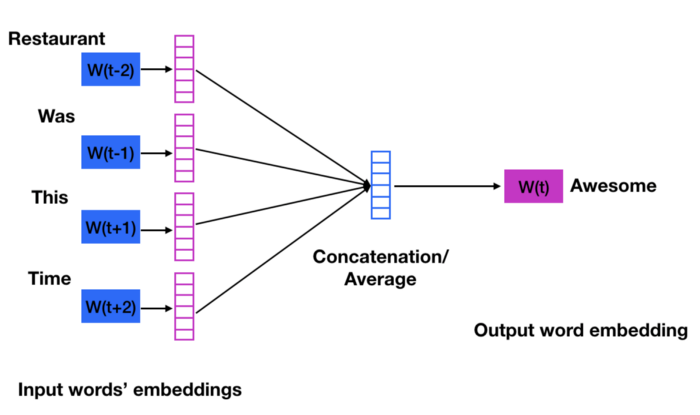
\includegraphics[scale=0.4]{images/cbow.png}
\caption{Arquitectura CBOW}
\end{figure}
\vspace{2mm}


\item \textbf{Skip Gram}: Es opuesto a CBOW, se predice las palabras más similares o alineadas para las palabras de contexto circundantes en la ventana específica dada una palabra actual.
A continuación se muestra el ejemplo anterior con un tamaño de ventana 2 para esta arquitectura:

\begin{figure}[htbp!]
\centering
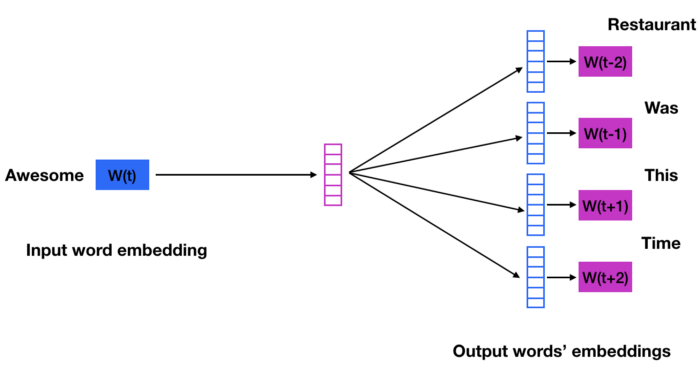
\includegraphics[scale=0.4]{images/skip.png}
\caption{Arquitectura Skip Gram}
\end{figure}
\vspace{2mm}

La capa de entrada contiene la palabra actual y la capa de salida contiene las palabras de contexto. La capa oculta contiene el número de dimensiones en las que queremos representar la palabra actual presente en la capa de entrada. 

\end{itemize}

\vspace{6mm}
{\setlength{\parindent}{0cm}
Centrándonos un poco más en nuestro problema a resolver:}
\vspace{2mm}\\
Los \textbf{vectores de palabras} también se pueden utilizar para \textbf{derivar clases de palabras} a partir de grandes conjuntos de datos. Esto se logra realizando \textbf{agrupaciones} de \textbf{K-medias} encima de los vectores de palabras. 
\vspace{2mm}\\
Podría resultarnos útil si se intenta agrupar todos los tweets con la misma polaridad para solventar de esta forma el problema de clasificación en función de la polaridad del documento. 


\subsection{Modelos de Deep Learning}


{\setlength{\parindent}{0cm}
Una buena aproximación que obtiene un \textit{accuracy} de 0.79 con una red neuronal de tipo LSTM es la que se encuentra en el siguiente enlace:\\ }
\url{https://www.kaggle.com/abhineethmishra/twitter-sentiment-analysis}\\
Utiliza junto con este tipo de redes el modelo \textit{word2vec} y además entrena con toda la colección completa. 
\vspace{2mm}\\
No he podido realizar pruebas con este tipo de hibridación ya que los tiempos de cómputo se disparaban. Sin embargo, para probar un poco \textit{word2vec} he realizado un pequeño experimento junto a una simple red de tipo FFNN con 3 capas, pero el \textit{accuracy} obtenido apenas superaba el 0.35.
\vspace{4mm}\\
Otra \textbf{aproximación} que he realizado está basada en el código: \\
\url{https://www.kaggle.com/oksanakalytenko/glove-lstm/notebook}\\
en el que se obtiene un \textit{accuracy} de 0.77 entrenando con toda la colección completa. \\Utiliza de forma similar a la anterior, redes neuronales \textbf{LSTM} pero \textbf{junto a Glove}, que es un \textit{word embedding} desarrollado por la Universidad de Standford.
\vspace{2mm}\\
\textbf{En mi caso he obtenido} un \textit{accuracy} de \textbf{0.71} entrenando con un subconjunto de entrenamiento del 3.75\% total (que son 60.000 instancias). Pese a utilizar tan pocos datos, ya tardó unos 42 minutos aprox. en ejecutar. La gráficas de aprendizaje obtenidas son:

\begin{wrapfigure}{r}{0.5\textwidth} %this figure will be at the right
    \centering
	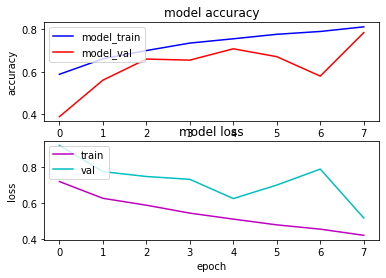
\includegraphics[scale=0.6]{images/av1.png}
    \caption{Gráficas de aprendizaje}
\end{wrapfigure}

\vspace{4mm}
Podemos observar que pese al parecer estar presente el sobreaprendizaje al inicio y en la sexta época de aprendizaje, al final ese incremento de rendimiento en training se ve reflejado en validación y no hay demasiada varianza o distancia entre ambas lineas, por lo que al final obtenemos un buen rendimiento del modelo entrenado.
\vspace{2mm}\\
Las redes LSTM al poder \textbf{retroalimentarse} pueden reaprender más rápidamente por ello obtenemos mejores resultados que con las FFNN del experimento anterior.


\chapter{Planteamiento de futuro}

Los enormes $datasets$ sobre opiniones y reseñas que se irán generando en las redes sociales (ya sea twitter, facebook o instagram) o en cualquier negocio online (como podría ser amazon) a lo largo de los años necesitarán de un
modelo de análisis de sentimiento \textbf{escalable} que sea lo suficientemente flexible
para ser aplicado a revisiones pertenecientes a diferentes ámbitos o dominios.

\section{Problemas que presenta el análisis de sentimientos}

{\setlength{\parindent}{0cm}
Algunos de los problemas que enunciaremos a continuación están directamente relacionados o podríamos decir que son problemas que se heredan del Procesamiento del Lenguaje Natural, entre ellos:}

\begin{itemize}
\item El sentimiento de las palabras a menudo depende del \textbf{contexto en el que estén ubicadas}, por ejemplo no tendría el mismo significado el verbo ``morir'' cuando nos referimos al fallecimiento de una persona (sentimientos negativos), que cuando utilizamos ``morir de la risa'' para denotar una situación graciosa (sentimientos positivos).

\item La \textbf{ambigüedad} es uno de los elementos lingüísticos más sutiles y complicados de resolver dentro del PLN. Las personas somos capaces de deducirlos dentro de un contexto y en base a nuestras experiencias, pero los ordenadores no cuentan con demasiados recursos para ello. Esto se complica cuando el nivel de granuralidad cada vez es más fino (análisis a nivel de aspecto y entidad).

\item  La \textbf{ironía} de las expresiones utilizadas por las personas o cualquier otra \textbf{expresión coloquial} que no se suele utilizar por mucha gente en general. 

\item Detección de las \textbf{frases negadas}, ya que palabras como ``no'' pueden invertir la polaridad del resto de palabras a las que acompañan (y no siempre la negación invierte el sentimiendo de éstas). 
\vspace{2mm}\\
Por ejemplo: ``La comida está buena'', si añadimos el ``no'' delante del verbo cambiaría totalmente la polaridad de ésta. 

Sin embargo, en la oración ``No cabe duda de que la comida está buenísima''`, sigue teniendo la polaridad positiva.

\end{itemize}

{\setlength{\parindent}{0cm}
En concreto, lo más relevante parece ser el contexto en el que se ubica el sentimiento y la interpretación que una persona pueda asociarle a dicha expresión, bien por la ambigüedad o por el dominio en el que se utilice.}
\vspace{2mm}\\
{\setlength{\parindent}{0cm}
Un estudio de Ogneva, M \cite{OGNEVA} sugiere que un \textit{accuracy} del 70\% exacto puede considerarse equivalente a como un humano percibe los sentimientos de otras personas, ya que esta percepción varía de una persona a otra. Incluso si el programa es produjese un $accuracy$ del 100\% correcto, los humanos
todavía no estarían de acuerdo con él en alrededor del 20\% de las predicciones.}


\section{¿Qué harías si puedes trabajar durante 6 meses en el problema?}

\begin{itemize}


\item Una idea: Captar la variada percepción de los humanos combinando gramáticas positivas y negativas sobre un
revisión subjetiva \cite{Bhuvan}, en nuestro caso podemos utilizar conjuntos de tweets que tengan una serie de hashtags asociados y estén relacionados con un tema específico. 
\vspace{2mm}\\
Los modelos de aprendizaje profundo, se pueden enriquecer aún más con estas representaciones semánticamente ricas utilizando \textbf{ontologías o gramáticas} para captar eficazmente la opinión de los tweets. Se podría trabajar en el futuro para experimentar con diferentes número de gramáticas y variaciones de extracción de características para no trabajar siempre con un vocabulario fijo.
\vspace{2mm}\\
Definir gramáticas es una sobrecarga adicional al ajuste del modelo, por lo tanto, se pueden realizar investigaciones para superar ésto haciendo modelos inteligentes que puedan aprender las gramáticas específicas al contexto.
\vspace{2mm}\\
Esto también hace que el modelo sea flexible ya que, ese \textbf{mismo modelo} se puede \textbf{usar} para \textbf{diferentes dominios} simplemente \textbf{definiendo nuevas gramáticas} específicas del contexto para ese dominio.

\item Otra idea sería realizar nuevos experimentos utilizando un enfoque \textbf{no supervisado} que se puede llevar a cabo utilizando el algoritmo de agrupación de $KMeans$ para encontrar el \textbf{punto de interrupción} sobre la puntuación de \textbf{opinión} en la que un tweet se clasifica como positivo o
negativo asumiendo un conjunto de datos distribuido uniformemente (asume implícitamente la misma importancia para cada gramática).
\vspace{2mm}\\
Para ello, una idea sería utilizar diferentes \textbf{pesos asociados} a los términos de cada una de las gramáticas, que denotaría su papel al describir el nivel de positividad o negatividad del tweet que se compara con la gramática. 
\vspace{2mm}\\
Los pesos \textbf{mostrarían cuán positivos o negativos} son dichos términos. Las exageraciones y las subestimaciones también podrían ser ponderadas. Para encontrar el peso más adecuado (óptimo) se podrían usar redes neuronales.

\end{itemize}

Aunque siempre habrá un sesgo asociado al $corpus$ o a la fuente de datos, no es posible que todos los documentos pertenecientes a ésta expresen de forma detallada el sentimiento. 


% BIBLIOGRAFIA
\begin{thebibliography}{0}

\bibitem{Jain} A. P. Jain and P. Dandannavar, ``Application of machine learning techniques to sentiment analysis,'' 2016 2nd International Conference on Applied and Theoretical Computing and Communication Technology (iCATccT), Bangalore, 2016.

\bibitem{Rokach} L. Rokach, Ensemble methods for classifiers, in: O. Maimon, L. Rokach (Eds.), Data Mining and Knowledge Discovery Handbook, Springer US, Boston,
MA, 2005

\bibitem{Kennedy} A. Kennedy, D. Inkpen, Sentiment classification of movie reviews using contextual valence shifters, Comput. Intell. 22 (2) (2006)

\bibitem{OGNEVA} Ogneva, M. ``How Companies Can Use Sentiment Analysis to Improve
Their Business''. Retrieved 2012-12-13.

\bibitem{Bhuvan} M. S. Bhuvan, V. D. Rao, S. Jain, T. S. Ashwin and R. M. R. Guddeti, ``Semantic sentiment analysis using context specific grammar'' International Conference on Computing, Communication \& Automation, Noida, 2015.
\vspace{6mm}\\
\textbf{Preprocesado}
\vspace{2mm}
\\\url{https://github.com/tthustla/twitter_sentiment_analysis_part1/blob/master/Capstone_part2.ipynb}
\vspace{2mm}
\\\url{https://medium.com/@himanshu_23732/sentiment-analysis-with-sentiment140-e6b0c789e0ce}
\vspace{2mm}
\\\url{http://openaccess.uoc.edu/webapps/o2/bitstream/10609/81435/6/jsobrinosTFM0618memoria.pdf}
\vspace{2mm}
\\\url{}
\vspace{2mm}\\
\\\textbf{Modelos Avanzados}
\vspace{2mm}
\\\url{https://code.google.com/archive/p/word2vec/}
\vspace{2mm}
\\\url{https://medium.com/swlh/sentiment-classification-using-word-embeddings-word2vec-aedf28fbb8ca}
\vspace{2mm}
\\\url{https://en.wikipedia.org/wiki/Long_short-term_memory}
\vspace{2mm}

  
\end{thebibliography}

\end{document}